\section{\ruby{付録}{ふ|ろく}:センサー紹介}\label{sensor_intr}
\subsection{デジタル出力装置}

\newlength{\colF}
\setlength{\colF}{0.25\columnwidth}
\newlength{\colG}
\setlength{\colG}{0.65\columnwidth}
\newlength{\colH}
\setlength{\colH}{0.1\columnwidth}
\newlength{\colI}
\setlength{\colI}{0.35\columnwidth}

\subsubsection{LED}\label{LED}
\begin{table}[H]
	\begin{tabular}{|p{\colF}|p{\colG}|}	\hline
	名称 & LED(えるいーでぃー)\\ \hline
	接続箇所 & デジタルコネクタ (3pin)\\ \hline
	機能概要 & LEDを点灯させる\\ \hline
  \end{tabular}
\end{table}

\begin{table}[H]
	\begin{tabular}{|p{\colF}|p{\colG}|}	\hline
	サンプルコードの場所 & 05/digout.hsp\\ \hline
	raspiへの入力 & なし\\ \hline
	raspiへの入力方法 & なし\\ \hline
	raspiからの出力 & 値が1の時点灯、値が0の時消灯\\ \hline
	raspiからの出力方法 & gpio GPIO番号, パラメータ\\ \hline
  \end{tabular}
\end{table}

\begin{table}[H]
	\begin{tabular}{|p{\colF}|p{\colG}|} \hline
	使い道 & 照明、信号機、車のライト\\ \hline
	注意事項 & なし\\ \hline
	補足 & プラスとマイナスの電荷がLEDチップ内で衝突するエネルギーを利用して発光します。LEDの光の色はLEDチップに含まれている半導体の種類で決まっています\\ \hline
  \end{tabular}
\end{table}

\begin{figure}[H]
	\begin{tabular}{|p{\colH}|p{\colI}|p{\colH}|p{\colI}|} \hline
	外観 & 
	\begin{minipage}[t]{\linewidth}
    \smallskip
      \centering
      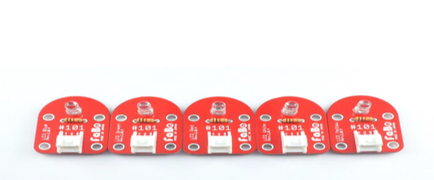
\includegraphics[width=\linewidth]{images/chap05/text05-img016.png}
      \caption{LED}
      \smallskip
    \end{minipage} &
    回路記号 & 
    \begin{minipage}[t]{\linewidth}
    \smallskip
      \centering
      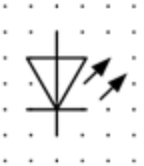
\includegraphics[width=\linewidth]{images/chap05/text05-img043.png}
      \caption{LEDの回路図}
      \smallskip
    \end{minipage}\\ \hline
  \end{tabular}
\end{figure}
